\scanpage{26}
% archive sheet number: 25
\[
\begin{aligned}
\langle C_{\eta},\operatorname{div} f_{\eta}\rangle_v
  &=i(C.\deleted{\overline{\operatorname{div} f_{\eta}}})\\
\rotatebox{90}{$=$}&\\
\unsure{=|\Leftrightarrow}\ v(f_{\eta}(C_{\eta}))&
\end{aligned}
\]
\diagram{\begin{tikzcd}[ampersand replacement=\&,column sep=small]
X'\arrow[r,hook,"\text{\unsure{imm. ouverte}}"] \& \widetilde X''\arrow[r,"\text{\uline{fini} \uline{\unsure{birat|birat.}}}"] \& X'' \arrow[r,phantom,"\overset{\text{\unsure{imm. fermée}}}{\subset}"] \& J
\end{tikzcd}}

\diagram{\begin{tikzcd}[ampersand replacement=\&,row sep=small]
X'\arrow[r,hook]\arrow[d,dash] \& J\\
S\&\\[-3pt]\&S
\end{tikzcd}}
\figure{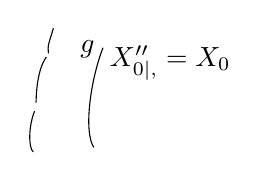
\begin{tikzpicture}[x=.45cm,y=.45cm]
\draw (0,2.8) .. controls (-.1,2.45) and (-.18,2.3) .. (-.14,2.09);
\draw (-.2,1.99) .. controls (-.43,1.65) and (-.48,1.12) .. (-.49,.7);
\draw (-.53,.46) .. controls (-.7,.05) and (-.71,-.57) .. (-.57,-.69);
\draw (1.4,2.25) .. controls (1.04,1.32) and (.85,-.12) .. (1.14,-.56);
\node at (.96,2.2) {$\deleted{\unsure{g}}$};
\node[anchor=west] at (1.32,1.83) {$X''_{\unsure{0|,}}=X_0$};
\end{tikzpicture}}
\diagram{\begin{tikzcd}[ampersand replacement=\&,row sep=small]
\unsure{K_{\eta}|k_{\eta}|X_{\eta}} \& X\arrow[d,dash]\\
\eta \& S\ \text{\unsure{spec. ann.} de val. discrète}
\end{tikzcd}}

\noindent\rule{2cm}{.4pt}

$x\in X_{\eta}(k(\eta))$\quad $\exists\ L$ faisceau loc. libre sur $X$ et une section rationnelle dont \deleted{\unsure{le|la}} diviseur sur $X_{\eta}$ est \unsure{réduit} : $(x)$

En \unsure{normalisant|modifiant}, on peut supposer que cette section est définie partout \uline{sauf} \unsure{en|au} \deleted{$x\in X_{\unsure{.}}$} le pt critique $x_0$, et que \deleted{elle \unsure{est}} son diviseur n'a pas de composante verticale. \unsure{Cela|Ceci} \unsure{que|car} \unsure{pour|que} la section donnée est un diviseur

\figure{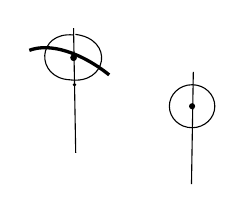
\begin{tikzpicture}[x=.78cm,y=.78cm]
\draw (0,1.58)--(.035,-.45);
\draw (0,1.47) .. controls (-.6,1.53) and (-.63,.77) .. (-.06,.74)
 .. controls (.55,.66) and (.67,1.4) .. (.03,1.48);
\draw[very thick] (-.72,1.22) .. controls (-.38,1.35) and (.13,1.18) .. (.58,.82);
\fill (0,1.10) circle (.055) (.015,.66) circle (.03);
\draw (1.95,.87)--(1.92,-.96);
\draw (1.93,.31) ellipse (.37 and .35);
\fill (1.93,.31) circle (.05);
\end{tikzpicture}}
